\section{The cf-transfer-v1 campaign}
\label{app:cf-transfer}

This appendix records the benchmark protocol as executed and the per-concept results of every completed block. The execution log with every acceptance decision, and the code, live in the \texttt{concept-flow} repository (branch \texttt{cf-transfer-mayo}, \texttt{docs/external-replication/}).

\subsection{Grid and consumed loci}
\label{app:cf-grid}

\begin{table}[h]
\centering\small
\caption{Checkpoints, consumed visual blocks (primary locus), and image strategy. All checkpoints run in bf16 with the pinned Hugging Face revision recorded in the code; the connector locus is the projector/merger output in every family.}
\label{tab:cf-grid}
\begin{tabular}{llll}
\toprule
Family & Sizes & Primary locus & Image strategy \\
\midrule
Qwen2.5-VL & 3B, 7B, 32B, 72B & \texttt{visual.blocks[-1]} (pre-merger) & $336^2$ pinned \\
Qwen3-VL & 4B, 8B, 32B & \texttt{visual.blocks[-1]} & max $512^2$ \\
InternVL3.5 & 8B, 14B, 38B & last InternViT layer (CLS excluded) & single $448^2$ tile \\
Gemma 3 & 4B, 12B, 27B & last SigLIP block (4096 tokens) & $896^2$ \\
MedGemma & 4B, 27B & last MedSigLIP block & $896^2$ \\
Lingshu & 7B, 32B & \texttt{visual.blocks[-1]} & $336^2$ pinned \\
LLaVA-1.5 & 7B, 13B & CLIP \texttt{layers[22]} (\texttt{hidden\_states[-2]}, CLS excluded) & $336^2$ \\
LLaVA-Med 1.5 & 7B & CLIP \texttt{layers[22]} (CLS excluded) & $336^2$ \\
Llama 3.2 Vision & 11B, 90B & last global transformer block (cross-attention) & single $560^2$ tile \\
\bottomrule
\end{tabular}
\end{table}

Each adapter records the module path, the consumed token mask, and any stream that bypasses the block (Llama~3.2 Vision's projector also reads five intermediate local-layer outputs; LLaVA's final CLIP block is computed but not consumed). Preflight check (C) verifies at run time that the write reaches the consumer and the answer logits and changes nothing outside the consumed tokens.

\subsection{Acceptance decisions}
\label{app:cf-gates}

All 57 completed blocks pass checks (A), (B), (C), and (G) with zero determinism error, zero change at $\alpha=0$, and fp32-versus-model logit differences below 0.13. Check (D) exceeds the 0.25-logit tolerance for the Qwen3-VL, Gemma~3, MedGemma, InternVL, and Llama families (up to 1.84 logits for Gemma~3 12B); these are recorded as declared deviations and neutralised by the fixed batch composition. Check (E) fails the A/B templates for LLaVA-1.5-7B and LLaVA-Med, the B-mapped templates for Qwen2.5-VL-3B and LLaVA-1.5-13B, and the yes/no and A-mapped templates for Llama~3.2 Vision 11B on all datasets; the affected cells are recorded as ineligible. Two checkpoints answer ``yes'' to nearly every chest question (Gemma~3 4B: clean $P(\mathrm{yes})>0.99$ on 94--97\% of rows), which the answerability grade records; three (LLaVA-1.5 7B/13B, LLaVA-Med) answer at chance.

\subsection{Coverage and cost}
\label{app:cf-coverage}

Eighteen checkpoints are complete on all three datasets with every module (CORE, CALIBRATION, PROMPT, DOSE, REFIT, LOCUS, LOCUS\_CALIBRATION on NIH and COCO; CORE and CALIBRATION on CheXpert); Llama~3.2 Vision 11B is complete with its yes/no modules ineligible; Qwen2.5-VL-72B is complete on NIH; the 72B COCO/CheXpert blocks, the 90B, and the remaining InternVL3.5-38B and Gemma~3 27B blocks are deferred or in progress at submission. The campaign consumed about 2,800 A100-hours on a Slurm cluster, with a file-locked task queue and automatic recovery of tasks killed at job time limits; every block's wall time is in its \texttt{run.json}.

\subsection{Seed replication details}
\label{app:cf-seed}

Qwen2.5-VL-7B on NIH: Effusion $W=0.190$, random p95 $=0.137$, $|\mathrm{sham}|=0.017$, rank 2 of 120, $O=-0.071$ $[-0.080,-0.062]$ with Nodule the maximiser; all six diagonals negative (Atelectasis $-0.226$, Pneumothorax $-0.102$, Cardiomegaly $-0.219$, Mass $-0.169$, Nodule $-0.072$). Mass wording: the mapping contrast IA$-$IB and the wording contrast IY$-$WY are reported for every block in the campaign tables; for the seed model Mass is owned under the \emph{show} A/B templates only, as in the original confirmation. Effusion does not transfer to CheXpert for the seed model ($W=0.08$, below the random p95).

\subsection{Per-concept results}
\label{app:cf-tables}

% Morandi tints for the cf-transfer tables (muted, low saturation); darker = larger value
\definecolor{cfSage1}{HTML}{EEF1EA}
\definecolor{cfSage2}{HTML}{D9E1D2}
\definecolor{cfSage3}{HTML}{C1CDB8}
\definecolor{cfSage4}{HTML}{A6B79C}
\definecolor{cfSlate1}{HTML}{ECEFF2}
\definecolor{cfSlate2}{HTML}{D3DAE2}
\definecolor{cfSlate3}{HTML}{B7C3D0}
\definecolor{cfSlate4}{HTML}{98A8B9}
\definecolor{cfTerra1}{HTML}{F5ECE9}
\definecolor{cfTerra2}{HTML}{E9D3CC}
\definecolor{cfTerra3}{HTML}{DAB5AA}
\definecolor{cfTerra4}{HTML}{C9968A}
\definecolor{cfOat1}{HTML}{F4EFE6}
\definecolor{cfOat2}{HTML}{E8DDC8}
\definecolor{cfGrey}{HTML}{E4E1DC}

\scriptsize
\setlength{\tabcolsep}{1.6pt}
\begin{longtable}{llrrccrrrrrll}
\caption{\textbf{NIH ChestX-ray14: every checkpoint--concept cell.} $S$: probe selectivity; AUROC: clean-answer AUROC; R/A: readable / answer-capable (\checkmark); $W_{qq}$: concept write; p95: random-family 95th percentile; $|$sham$|$; $O_q$ with 95\% percentile interval; rank of $W_{qq}$ among the 120 compared effects; strongest competitor; max-$T$ verdict. Owned rows are shaded slate.}\\
\label{tab:cf-nih}\\
\toprule
Checkpoint & Concept & $S$ & AUROC & R & A & $W_{qq}$ & p95 & $|$sham$|$ & $O_q$ & 95\% CI & Competitor & Verdict \\
\midrule
\endfirsthead
\toprule
Checkpoint & Concept & $S$ & AUROC & R & A & $W_{qq}$ & p95 & $|$sham$|$ & $O_q$ & 95\% CI & Competitor & Verdict \\
\midrule
\endhead
\midrule\multicolumn{13}{r}{\emph{continued}}\\
\endfoot
\bottomrule
\endlastfoot
Qwen2.5-VL-3B & Effusion & 0.137 & 0.582 & $\checkmark$ &  & -0.040 & 0.083 & 0.023 & -0.094 & [-0.10, -0.09] & Cardiomegaly & competitor \\
Qwen2.5-VL-3B & Atelectasis & 0.046 & 0.535 &  &  & -0.011 & 0.043 & 0.090 & -0.038 & [-0.04, -0.04] & Nodule & competitor \\
Qwen2.5-VL-3B & Pneumothorax & 0.104 & 0.432 &  &  & -0.057 & 0.139 & 0.110 & -0.176 & [-0.18, -0.17] & Mass & competitor \\
Qwen2.5-VL-3B & Cardiomegaly & 0.137 & 0.615 & $\checkmark$ &  & +0.051 & 0.192 & 0.120 & -0.109 & [-0.11, -0.11] & Atelectasis & competitor \\
Qwen2.5-VL-3B & Mass & 0.061 & 0.682 &  & $\checkmark$ & +0.148 & 0.177 & 0.261 & -0.040 & [-0.04, -0.04] & Atelectasis & competitor \\
Qwen2.5-VL-3B & Nodule & -0.039 & 0.608 &  & $\checkmark$ & +0.137 & 0.164 & 0.073 & -0.035 & [-0.04, -0.03] & Atelectasis & competitor \\
Qwen2.5-VL-7B & Effusion & 0.102 & 0.593 & $\checkmark$ &  & +0.190 & 0.137 & 0.017 & -0.071 & [-0.08, -0.06] & Nodule & competitor \\
Qwen2.5-VL-7B & Atelectasis & 0.062 & 0.566 &  &  & +0.101 & 0.297 & 0.096 & -0.226 & [-0.23, -0.22] & Nodule & competitor \\
Qwen2.5-VL-7B & Pneumothorax & 0.152 & 0.508 & $\checkmark$ &  & +0.089 & 0.320 & 0.113 & -0.102 & [-0.11, -0.10] & Effusion & competitor \\
Qwen2.5-VL-7B & Cardiomegaly & 0.205 & 0.742 & $\checkmark$ & $\checkmark$ & +0.085 & 0.311 & 0.158 & -0.219 & [-0.23, -0.21] & Atelectasis & competitor \\
Qwen2.5-VL-7B & Mass & 0.021 & 0.678 &  & $\checkmark$ & +0.359 & 0.372 & 0.092 & -0.169 & [-0.18, -0.16] & Effusion & competitor \\
Qwen2.5-VL-7B & Nodule & -0.041 & 0.642 &  & $\checkmark$ & +0.118 & 0.158 & 0.055 & -0.072 & [-0.08, -0.06] & Effusion & competitor \\
Qwen2.5-VL-32B & Effusion & 0.075 & 0.470 &  &  & -0.041 & 0.076 & 0.040 & -0.218 & [-0.23, -0.20] & Nodule & competitor \\
Qwen2.5-VL-32B & Atelectasis & 0.080 & 0.616 & $\checkmark$ & $\checkmark$ & +0.034 & 0.049 & 0.097 & -0.059 & [-0.07, -0.05] & Mass & competitor \\
Qwen2.5-VL-32B & Pneumothorax & 0.140 & 0.623 & $\checkmark$ &  & +0.032 & 0.053 & 0.075 & -0.056 & [-0.06, -0.05] & Cardiomegaly & competitor \\
\rowcolor{cfSlate2}Qwen2.5-VL-32B & Cardiomegaly & 0.171 & 0.670 & $\checkmark$ & $\checkmark$ & +0.192 & 0.082 & 0.043 & +0.106 & [+0.10, +0.12] & Nodule & owned \\
Qwen2.5-VL-32B & Mass & 0.069 & 0.769 &  & $\checkmark$ & +0.165 & 0.231 & 0.047 & -0.077 & [-0.09, -0.06] & Cardiomegaly & competitor \\
Qwen2.5-VL-32B & Nodule & 0.034 & 0.662 &  & $\checkmark$ & +0.009 & 0.132 & 0.001 & -0.051 & [-0.06, -0.05] & Mass & competitor \\
Qwen2.5-VL-72B & Effusion & 0.041 & 0.624 &  & $\checkmark$ & -0.011 & 0.201 & 0.084 & -0.322 & [-0.33, -0.32] & Atelectasis & competitor \\
\rowcolor{cfSlate2}Qwen2.5-VL-72B & Atelectasis & 0.072 & 0.573 &  &  & +0.531 & 0.213 & 0.015 & +0.537 & [+0.53, +0.54] & Cardiomegaly & owned \\
Qwen2.5-VL-72B & Pneumothorax & 0.136 & 0.478 & $\checkmark$ &  & -0.015 & 0.389 & 0.087 & -0.498 & [-0.50, -0.49] & Atelectasis & competitor \\
\rowcolor{cfSlate2}Qwen2.5-VL-72B & Cardiomegaly & 0.192 & 0.659 & $\checkmark$ & $\checkmark$ & +0.462 & 0.408 & 0.107 & +0.256 & [+0.25, +0.26] & Atelectasis & owned \\
\rowcolor{cfSlate2}Qwen2.5-VL-72B & Mass & 0.031 & 0.685 &  & $\checkmark$ & +0.328 & 0.292 & 0.005 & +0.066 & [+0.05, +0.08] & Atelectasis & owned \\
Qwen2.5-VL-72B & Nodule & -0.025 & 0.679 &  & $\checkmark$ & -0.016 & 0.144 & 0.069 & -0.230 & [-0.24, -0.22] & Mass & competitor \\
Qwen3-VL-4B & Effusion & 0.098 & 0.769 & $\checkmark$ & $\checkmark$ & +0.386 & 0.289 & 0.099 & -0.026 & [-0.04, -0.01] & Atelectasis & competitor \\
Qwen3-VL-4B & Atelectasis & 0.102 & 0.639 & $\checkmark$ & $\checkmark$ & +0.139 & 0.225 & 0.066 & -0.071 & [-0.08, -0.06] & Effusion & competitor \\
Qwen3-VL-4B & Pneumothorax & 0.062 & 0.672 &  & $\checkmark$ & +0.002 & 0.047 & 0.023 & -0.287 & [-0.31, -0.26] & Atelectasis & competitor \\
Qwen3-VL-4B & Cardiomegaly & 0.139 & 0.726 & $\checkmark$ & $\checkmark$ & +0.269 & 0.397 & 0.308 & -0.084 & [-0.10, -0.07] & Effusion & competitor \\
Qwen3-VL-4B & Mass & 0.112 & 0.785 &  & $\checkmark$ & -0.004 & 0.097 & 0.008 & -0.135 & [-0.15, -0.12] & Effusion & competitor \\
Qwen3-VL-4B & Nodule & -0.050 & 0.655 &  & $\checkmark$ & -0.011 & 0.056 & 0.004 & -0.086 & [-0.10, -0.07] & Cardiomegaly & competitor \\
Qwen3-VL-8B & Effusion & 0.128 & 0.766 & $\checkmark$ & $\checkmark$ & +0.232 & 0.360 & 0.024 & +0.073 & [+0.05, +0.10] & Nodule & no reference \\
Qwen3-VL-8B & Atelectasis & 0.069 & 0.653 &  & $\checkmark$ & +0.036 & 0.049 & 0.048 & -0.012 & [-0.01, -0.01] & Cardiomegaly & competitor \\
Qwen3-VL-8B & Pneumothorax & 0.127 & 0.656 & $\checkmark$ & $\checkmark$ & +0.052 & 0.168 & 0.008 & -0.067 & [-0.07, -0.06] & Mass & competitor \\
Qwen3-VL-8B & Cardiomegaly & 0.202 & 0.799 & $\checkmark$ & $\checkmark$ & +0.177 & 0.177 & 0.175 & +0.000 & [+0.00, +0.00] & Nodule & unresolved \\
Qwen3-VL-8B & Mass & 0.124 & 0.641 & $\checkmark$ & $\checkmark$ & -0.054 & 0.208 & 0.165 & -0.107 & [-0.13, -0.09] & Nodule & competitor \\
Qwen3-VL-8B & Nodule & -0.070 & 0.651 &  & $\checkmark$ & -0.050 & 0.189 & 0.103 & +0.035 & [+0.02, +0.05] & Effusion & no reference \\
Qwen3-VL-32B & Effusion & 0.089 & 0.713 &  & $\checkmark$ & -0.012 & 0.061 & 0.038 & -0.140 & [-0.16, -0.12] & Nodule & competitor \\
Qwen3-VL-32B & Atelectasis & 0.125 & 0.674 & $\checkmark$ & $\checkmark$ & +0.074 & 0.123 & 0.012 & -0.039 & [-0.04, -0.03] & Mass & competitor \\
Qwen3-VL-32B & Pneumothorax & 0.115 & 0.684 &  & $\checkmark$ & +0.008 & 0.005 & 0.001 & +0.003 & [-0.00, +0.01] & Mass & unresolved \\
Qwen3-VL-32B & Cardiomegaly & 0.189 & 0.709 & $\checkmark$ & $\checkmark$ & +0.136 & 0.238 & 0.030 & -0.039 & [-0.05, -0.02] & Nodule & competitor \\
Qwen3-VL-32B & Mass & 0.082 & 0.780 &  & $\checkmark$ & +0.091 & 0.093 & 0.015 & -0.106 & [-0.12, -0.09] & Nodule & competitor \\
\rowcolor{cfSlate2}Qwen3-VL-32B & Nodule & -0.013 & 0.612 &  & $\checkmark$ & +0.242 & 0.116 & 0.038 & +0.171 & [+0.16, +0.19] & Mass & owned \\
InternVL3.5-8B & Effusion & 0.074 & 0.771 &  & $\checkmark$ & +0.008 & 0.013 & 0.006 & +0.003 & [+0.00, +0.00] & Mass & no reference \\
InternVL3.5-8B & Atelectasis & 0.045 & 0.710 &  & $\checkmark$ & -0.004 & 0.028 & 0.005 & -0.015 & [-0.02, -0.01] & Effusion & competitor \\
InternVL3.5-8B & Pneumothorax & 0.062 & 0.701 &  & $\checkmark$ & +0.001 & 0.003 & 0.002 & -0.000 & [-0.00, -0.00] & Mass & unresolved \\
InternVL3.5-8B & Cardiomegaly & 0.135 & 0.753 & $\checkmark$ & $\checkmark$ & +0.035 & 0.062 & 0.032 & +0.002 & [-0.00, +0.00] & Pneumothorax & unresolved \\
InternVL3.5-8B & Mass & 0.109 & 0.780 & $\checkmark$ & $\checkmark$ & +0.011 & 0.019 & 0.009 & -0.006 & [-0.01, -0.00] & Pneumothorax & competitor \\
InternVL3.5-8B & Nodule & -0.057 & 0.664 &  & $\checkmark$ & +0.007 & 0.023 & 0.029 & -0.014 & [-0.02, -0.01] & Pneumothorax & competitor \\
\rowcolor{cfSlate2}InternVL3.5-14B & Effusion & 0.125 & 0.790 & $\checkmark$ & $\checkmark$ & +0.012 & 0.009 & 0.008 & +0.009 & [+0.01, +0.01] & Atelectasis & owned \\
InternVL3.5-14B & Atelectasis & 0.086 & 0.726 & $\checkmark$ & $\checkmark$ & -0.000 & 0.024 & 0.009 & -0.010 & [-0.01, -0.01] & Mass & competitor \\
InternVL3.5-14B & Pneumothorax & 0.093 & 0.721 & $\checkmark$ & $\checkmark$ & -0.000 & 0.001 & 0.000 & -0.000 & [-0.00, -0.00] & Mass & unresolved \\
InternVL3.5-14B & Cardiomegaly & 0.182 & 0.777 & $\checkmark$ & $\checkmark$ & +0.021 & 0.037 & 0.029 & -0.005 & [-0.01, -0.00] & Nodule & unresolved \\
InternVL3.5-14B & Mass & 0.031 & 0.744 &  & $\checkmark$ & +0.007 & 0.011 & 0.007 & +0.005 & [+0.00, +0.01] & Cardiomegaly & no reference \\
InternVL3.5-14B & Nodule & -0.076 & 0.647 &  & $\checkmark$ & -0.002 & 0.019 & 0.004 & -0.009 & [-0.01, -0.01] & Mass & competitor \\
Gemma 3 4B & Effusion & 0.080 & 0.561 &  &  & -0.005 & 0.000 & 0.085 & -0.004 & [-0.01, +0.00] & Cardiomegaly & unresolved \\
Gemma 3 4B & Atelectasis & 0.107 & 0.535 & $\checkmark$ &  & -0.002 & -0.000 & 0.000 & -0.002 & [-0.00, -0.00] & Effusion & unresolved \\
Gemma 3 4B & Pneumothorax & -0.044 & 0.595 &  &  & -0.005 & 0.011 & 0.009 & -0.014 & [-0.02, -0.01] & Cardiomegaly & competitor \\
Gemma 3 4B & Cardiomegaly & 0.086 & 0.627 &  & $\checkmark$ & -0.252 & 0.001 & 0.034 & -0.238 & [-0.27, -0.21] & Effusion & competitor \\
Gemma 3 4B & Mass & 0.061 & 0.643 &  & $\checkmark$ & -0.344 & 0.144 & 0.130 & -0.276 & [-0.32, -0.23] & Effusion & competitor \\
Gemma 3 4B & Nodule & 0.140 & 0.414 & $\checkmark$ &  & -0.146 & 0.024 & 0.272 & -0.122 & [-0.15, -0.09] & Cardiomegaly & competitor \\
Gemma 3 12B & Effusion & 0.080 & 0.648 &  & $\checkmark$ & -0.280 & 0.511 & 0.287 & -0.834 & [-0.86, -0.81] & Nodule & competitor \\
Gemma 3 12B & Atelectasis & 0.107 & 0.659 & $\checkmark$ & $\checkmark$ & -0.347 & 0.231 & 0.058 & -0.569 & [-0.60, -0.53] & Nodule & competitor \\
Gemma 3 12B & Pneumothorax & -0.044 & 0.660 &  & $\checkmark$ & +0.098 & 0.627 & 0.028 & -0.172 & [-0.21, -0.13] & Cardiomegaly & competitor \\
Gemma 3 12B & Cardiomegaly & 0.086 & 0.516 &  &  & +0.329 & 0.738 & 0.334 & -0.194 & [-0.24, -0.15] & Nodule & competitor \\
Gemma 3 12B & Mass & 0.061 & 0.633 &  & $\checkmark$ & -0.177 & 0.501 & 0.550 & -0.647 & [-0.68, -0.62] & Nodule & competitor \\
\rowcolor{cfSlate2}Gemma 3 12B & Nodule & 0.140 & 0.634 & $\checkmark$ & $\checkmark$ & +0.385 & 0.369 & 0.151 & +0.167 & [+0.14, +0.20] & Pneumothorax & owned \\
Gemma 3 27B & Effusion & 0.078 & 0.583 &  &  & +0.208 & 0.271 & 0.226 & -0.044 & [-0.06, -0.03] & Mass & competitor \\
Gemma 3 27B & Atelectasis & 0.110 & 0.592 & $\checkmark$ & $\checkmark$ & -0.022 & 0.005 & 0.005 & -0.028 & [-0.04, -0.02] & Cardiomegaly & competitor \\
Gemma 3 27B & Pneumothorax & -0.040 & 0.590 &  &  & +0.375 & 0.397 & 0.129 & -0.012 & [-0.02, -0.00] & Mass & unresolved \\
Gemma 3 27B & Cardiomegaly & 0.086 & 0.601 &  &  & +0.045 & 0.045 & 0.045 & +0.002 & [+0.00, +0.00] & Nodule & unresolved \\
Gemma 3 27B & Mass & 0.061 & 0.649 &  & $\checkmark$ & +0.096 & 0.185 & 0.187 & -0.078 & [-0.09, -0.06] & Cardiomegaly & competitor \\
Gemma 3 27B & Nodule & 0.141 & 0.608 & $\checkmark$ & $\checkmark$ & +0.047 & 0.067 & 0.058 & -0.016 & [-0.02, -0.01] & Effusion & competitor \\
MedGemma 4B & Effusion & 0.108 & 0.803 &  & $\checkmark$ & +0.084 & 0.133 & 0.377 & +0.005 & [-0.02, +0.03] & Nodule & unresolved \\
MedGemma 4B & Atelectasis & 0.138 & 0.784 & $\checkmark$ & $\checkmark$ & -0.358 & 0.179 & 0.138 & -0.558 & [-0.59, -0.52] & Pneumothorax & competitor \\
MedGemma 4B & Pneumothorax & 0.109 & 0.823 &  & $\checkmark$ & +0.044 & 0.194 & 0.012 & +0.005 & [-0.01, +0.02] & Atelectasis & unresolved \\
MedGemma 4B & Cardiomegaly & 0.198 & 0.894 & $\checkmark$ & $\checkmark$ & +0.192 & 0.370 & 0.104 & -0.067 & [-0.11, -0.03] & Pneumothorax & competitor \\
MedGemma 4B & Mass & 0.168 & 0.834 & $\checkmark$ & $\checkmark$ & -0.100 & 0.318 & 0.033 & -0.273 & [-0.31, -0.24] & Nodule & competitor \\
MedGemma 4B & Nodule & 0.016 & 0.666 &  & $\checkmark$ & +0.129 & 0.542 & 0.551 & +0.094 & [+0.07, +0.12] & Atelectasis & no reference \\
MedGemma 27B & Effusion & 0.107 & 0.855 &  & $\checkmark$ & -0.012 & 0.057 & 0.040 & -0.064 & [-0.08, -0.05] & Pneumothorax & competitor \\
MedGemma 27B & Atelectasis & 0.138 & 0.755 & $\checkmark$ & $\checkmark$ & -0.331 & 0.116 & 0.292 & -0.446 & [-0.48, -0.41] & Cardiomegaly & competitor \\
MedGemma 27B & Pneumothorax & 0.109 & 0.799 &  & $\checkmark$ & -0.005 & 0.050 & 0.062 & -0.013 & [-0.02, -0.00] & Nodule & unresolved \\
MedGemma 27B & Cardiomegaly & 0.197 & 0.871 & $\checkmark$ & $\checkmark$ & +0.645 & 0.646 & 0.583 & +0.002 & [+0.00, +0.00] & Pneumothorax & no reference \\
MedGemma 27B & Mass & 0.168 & 0.860 & $\checkmark$ & $\checkmark$ & -0.091 & 0.044 & 0.034 & -0.132 & [-0.15, -0.12] & Pneumothorax & competitor \\
MedGemma 27B & Nodule & 0.016 & 0.662 &  & $\checkmark$ & -0.120 & 0.190 & 0.151 & -0.203 & [-0.23, -0.18] & Atelectasis & competitor \\
Lingshu 7B & Effusion & 0.120 & 0.780 & $\checkmark$ & $\checkmark$ & +0.066 & 0.078 & 0.064 & +0.018 & [+0.01, +0.03] & Cardiomegaly & no reference \\
Lingshu 7B & Atelectasis & 0.102 & 0.748 & $\checkmark$ & $\checkmark$ & +0.099 & 0.117 & 0.052 & +0.014 & [+0.01, +0.02] & Nodule & no reference \\
Lingshu 7B & Pneumothorax & 0.096 & 0.796 &  & $\checkmark$ & +0.070 & 0.101 & 0.032 & +0.010 & [+0.00, +0.02] & Nodule & unresolved \\
\rowcolor{cfSlate2}Lingshu 7B & Cardiomegaly & 0.234 & 0.778 & $\checkmark$ & $\checkmark$ & +0.222 & 0.117 & 0.040 & +0.170 & [+0.16, +0.18] & Nodule & owned \\
Lingshu 7B & Mass & 0.008 & 0.809 &  & $\checkmark$ & +0.029 & 0.135 & 0.041 & -0.086 & [-0.09, -0.08] & Nodule & competitor \\
Lingshu 7B & Nodule & -0.075 & 0.656 &  & $\checkmark$ & +0.066 & 0.103 & 0.130 & +0.016 & [+0.01, +0.02] & Cardiomegaly & no reference \\
Lingshu 32B & Effusion & 0.111 & 0.789 & $\checkmark$ & $\checkmark$ & +0.060 & 0.063 & 0.047 & -0.007 & [-0.01, -0.00] & Mass & unresolved \\
Lingshu 32B & Atelectasis & 0.096 & 0.739 & $\checkmark$ & $\checkmark$ & +0.021 & 0.074 & 0.013 & -0.080 & [-0.09, -0.07] & Pneumothorax & competitor \\
\rowcolor{cfSlate2}Lingshu 32B & Pneumothorax & 0.137 & 0.818 & $\checkmark$ & $\checkmark$ & +0.202 & 0.065 & 0.051 & +0.144 & [+0.14, +0.15] & Mass & owned \\
\rowcolor{cfSlate2}Lingshu 32B & Cardiomegaly & 0.072 & 0.860 &  & $\checkmark$ & +0.105 & 0.086 & 0.014 & +0.051 & [+0.04, +0.06] & Mass & owned \\
Lingshu 32B & Mass & 0.102 & 0.861 &  & $\checkmark$ & +0.065 & 0.069 & 0.011 & -0.077 & [-0.08, -0.07] & Pneumothorax & competitor \\
Lingshu 32B & Nodule & -0.066 & 0.642 &  & $\checkmark$ & -0.086 & 0.061 & 0.043 & -0.178 & [-0.19, -0.17] & Pneumothorax & competitor \\
LLaVA-1.5-7B & Effusion & 0.110 & 0.405 & $\checkmark$ &  & +0.038 & 0.094 & 0.058 & -0.028 & [-0.03, -0.03] & Mass & competitor \\
LLaVA-1.5-7B & Atelectasis & 0.102 & 0.569 & $\checkmark$ &  & +0.042 & 0.089 & 0.028 & -0.015 & [-0.02, -0.01] & Mass & competitor \\
LLaVA-1.5-7B & Pneumothorax & 0.104 & 0.509 &  &  & -0.033 & 0.082 & 0.076 & -0.080 & [-0.08, -0.08] & Mass & competitor \\
LLaVA-1.5-7B & Cardiomegaly & 0.053 & 0.519 &  &  & -0.032 & 0.104 & 0.013 & -0.133 & [-0.14, -0.13] & Effusion & competitor \\
LLaVA-1.5-7B & Mass & 0.087 & 0.534 &  &  & +0.049 & 0.056 & 0.037 & +0.023 & [+0.02, +0.03] & Nodule & no reference \\
LLaVA-1.5-7B & Nodule & 0.031 & 0.506 &  &  & +0.010 & 0.047 & 0.008 & -0.018 & [-0.02, -0.02] & Mass & competitor \\
LLaVA-1.5-13B & Effusion & 0.110 & 0.506 & $\checkmark$ &  & +0.003 & 0.057 & 0.042 & -0.013 & [-0.02, -0.01] & Mass & competitor \\
LLaVA-1.5-13B & Atelectasis & 0.102 & 0.554 & $\checkmark$ &  & -0.045 & 0.021 & 0.012 & -0.047 & [-0.05, -0.04] & Nodule & competitor \\
LLaVA-1.5-13B & Pneumothorax & 0.104 & 0.564 &  &  & -0.019 & 0.036 & 0.036 & -0.037 & [-0.04, -0.03] & Nodule & competitor \\
LLaVA-1.5-13B & Cardiomegaly & 0.053 & 0.488 &  &  & -0.004 & 0.058 & 0.015 & -0.029 & [-0.03, -0.03] & Mass & competitor \\
LLaVA-1.5-13B & Mass & 0.087 & 0.548 &  &  & +0.018 & 0.032 & 0.015 & +0.008 & [+0.01, +0.01] & Cardiomegaly & no reference \\
LLaVA-1.5-13B & Nodule & 0.031 & 0.525 &  &  & +0.001 & 0.026 & 0.022 & -0.015 & [-0.02, -0.01] & Cardiomegaly & competitor \\
LLaVA-Med 1.5 7B & Effusion & 0.119 & 0.525 & $\checkmark$ &  & +0.004 & 0.008 & 0.001 & -0.001 & [-0.00, -0.00] & Mass & competitor \\
LLaVA-Med 1.5 7B & Atelectasis & 0.105 & 0.517 & $\checkmark$ &  & +0.002 & 0.007 & 0.001 & -0.004 & [-0.00, -0.00] & Mass & competitor \\
LLaVA-Med 1.5 7B & Pneumothorax & 0.110 & 0.483 & $\checkmark$ &  & -0.021 & 0.018 & 0.018 & -0.038 & [-0.04, -0.04] & Cardiomegaly & competitor \\
LLaVA-Med 1.5 7B & Cardiomegaly & 0.061 & 0.583 &  &  & +0.024 & 0.034 & 0.023 & -0.010 & [-0.01, -0.01] & Effusion & competitor \\
LLaVA-Med 1.5 7B & Mass & 0.085 & 0.553 &  &  & +0.008 & 0.012 & 0.003 & -0.007 & [-0.01, -0.01] & Effusion & competitor \\
LLaVA-Med 1.5 7B & Nodule & 0.019 & 0.530 &  &  & -0.009 & 0.011 & 0.013 & -0.021 & [-0.02, -0.02] & Effusion & competitor \\
Llama 3.2 Vision 11B & Effusion & 0.128 & -- & $\checkmark$ & & -- & -- & -- & -- & -- & -- & ineligible \\
Llama 3.2 Vision 11B & Atelectasis & 0.054 & -- &  & & -- & -- & -- & -- & -- & -- & ineligible \\
Llama 3.2 Vision 11B & Pneumothorax & 0.150 & -- & $\checkmark$ & & -- & -- & -- & -- & -- & -- & ineligible \\
Llama 3.2 Vision 11B & Cardiomegaly & 0.118 & -- &  & & -- & -- & -- & -- & -- & -- & ineligible \\
Llama 3.2 Vision 11B & Mass & 0.001 & -- &  & & -- & -- & -- & -- & -- & -- & ineligible \\
Llama 3.2 Vision 11B & Nodule & 0.003 & -- &  & & -- & -- & -- & -- & -- & -- & ineligible \\
\end{longtable}
\normalsize

\begin{longtable}{llrrrrrl}
\caption{\textbf{CheXpert Plus: per-concept results of the external replication.} $S$: probe selectivity; ans.\ AUROC: clean-answer AUROC; $W_{qq}$: mean change in $P(\mathrm{yes})$ under the concept write; $O_q$: ownership contrast; p95: 95th percentile of the 119 random-direction writes; verdict from the simultaneous max-$T$ bounds (own = steering reference met and every lower bound $>0$).}\\
\label{tab:cf-chexpert}\\
\toprule
Checkpoint & Concept & $S$ & ans.\ AUROC & $W_{qq}$ & $O_q$ & p95 & Verdict \\
\midrule
\endfirsthead
\toprule
Checkpoint & Concept & $S$ & ans.\ AUROC & $W_{qq}$ & $O_q$ & p95 & Verdict \\
\midrule
\endhead
Qwen2.5-VL-3B & Effusion & 0.228 & 0.658 & -0.191 & -0.178 & 0.063 & competitor \\
Qwen2.5-VL-3B & Atelectasis & 0.171 & 0.619 & -0.018 & -0.016 & 0.059 & competitor \\
Qwen2.5-VL-3B & Pneumothorax & 0.005 & 0.446 & -0.034 & -0.044 & 0.106 & competitor \\
Qwen2.5-VL-3B & Cardiomegaly & 0.256 & 0.634 & 0.026 & -0.054 & 0.156 & competitor \\
Qwen2.5-VL-3B & Consolidation & 0.180 & 0.573 & -0.002 & -0.026 & 0.060 & competitor \\
Qwen2.5-VL-3B & Edema & 0.185 & 0.506 & -0.021 & -0.083 & 0.133 & competitor \\
Qwen2.5-VL-7B & Effusion & 0.234 & 0.676 & 0.075 & 0.008 & 0.114 & no ref. \\
Qwen2.5-VL-7B & Atelectasis & 0.351 & 0.851 & 0.208 & -0.049 & 0.266 & competitor \\
Qwen2.5-VL-7B & Pneumothorax & -0.028 & 0.606 & 0.106 & -0.099 & 0.372 & competitor \\
Qwen2.5-VL-7B & Cardiomegaly & 0.243 & 0.693 & 0.140 & -0.004 & 0.213 & unresolved \\
Qwen2.5-VL-7B & Consolidation & 0.203 & 0.565 & 0.119 & -0.149 & 0.245 & competitor \\
Qwen2.5-VL-7B & Edema & 0.178 & 0.520 & 0.040 & -0.177 & 0.212 & competitor \\
Qwen2.5-VL-32B & Effusion & 0.240 & 0.681 & -0.069 & -0.066 & 0.125 & competitor \\
Qwen2.5-VL-32B & Atelectasis & 0.065 & 0.925 & -0.146 & -0.187 & 0.029 & competitor \\
Qwen2.5-VL-32B & Pneumothorax & 0.060 & 0.532 & 0.021 & -0.124 & 0.088 & competitor \\
Qwen2.5-VL-32B & Cardiomegaly & 0.220 & 0.732 & -0.159 & -0.186 & 0.077 & competitor \\
Qwen2.5-VL-32B & Consolidation & 0.198 & 0.704 & -0.003 & -0.053 & 0.157 & competitor \\
Qwen2.5-VL-32B & Edema & 0.187 & 0.647 & -0.005 & -0.022 & 0.084 & competitor \\
Qwen3-VL-4B & Effusion & 0.230 & 0.898 & 0.398 & -0.015 & 0.308 & competitor \\
Qwen3-VL-4B & Atelectasis & 0.278 & 0.657 & 0.026 & -0.016 & 0.034 & competitor \\
Qwen3-VL-4B & Pneumothorax & 0.049 & 0.451 & 0.015 & -0.231 & 0.282 & competitor \\
Qwen3-VL-4B & Cardiomegaly & 0.246 & 0.854 & 0.098 & -0.008 & 0.104 & competitor \\
Qwen3-VL-4B & Consolidation & 0.245 & 0.789 & 0.807 & 0.094 & 0.428 & own \\
Qwen3-VL-4B & Edema & 0.176 & 0.816 & 0.593 & 0.092 & 0.426 & own \\
Qwen3-VL-8B & Effusion & 0.226 & 0.889 & 0.370 & -0.069 & 0.296 & competitor \\
Qwen3-VL-8B & Atelectasis & 0.164 & 0.791 & 0.009 & -0.000 & 0.009 & competitor \\
Qwen3-VL-8B & Pneumothorax & 0.062 & 0.466 & 0.203 & -0.095 & 0.390 & competitor \\
Qwen3-VL-8B & Cardiomegaly & 0.218 & 0.766 & 0.072 & -0.000 & 0.072 & competitor \\
Qwen3-VL-8B & Consolidation & 0.213 & 0.798 & 0.352 & -0.038 & 0.315 & competitor \\
Qwen3-VL-8B & Edema & 0.162 & 0.787 & 0.333 & -0.061 & 0.375 & competitor \\
Qwen3-VL-32B & Effusion & 0.237 & 0.899 & 0.083 & -0.035 & 0.151 & competitor \\
Qwen3-VL-32B & Atelectasis & 0.065 & 0.899 & 0.023 & 0.001 & 0.023 & unresolved \\
Qwen3-VL-32B & Pneumothorax & 0.130 & 0.607 & 0.011 & 0.001 & 0.018 & unresolved \\
Qwen3-VL-32B & Cardiomegaly & 0.243 & 0.862 & 0.091 & -0.026 & 0.117 & competitor \\
Qwen3-VL-32B & Consolidation & 0.191 & 0.878 & 0.024 & -0.124 & 0.103 & competitor \\
Qwen3-VL-32B & Edema & 0.161 & 0.782 & 0.237 & 0.045 & 0.187 & own \\
InternVL3.5-8B & Effusion & 0.253 & 0.946 & 0.011 & -0.006 & 0.028 & competitor \\
InternVL3.5-8B & Atelectasis & 0.211 & 0.918 & -0.007 & -0.014 & 0.012 & competitor \\
InternVL3.5-8B & Pneumothorax & -0.000 & 0.630 & 0.004 & 0.004 & 0.004 & own \\
InternVL3.5-8B & Cardiomegaly & 0.217 & 0.930 & 0.038 & -0.005 & 0.056 & competitor \\
InternVL3.5-8B & Consolidation & 0.256 & 0.932 & 0.022 & 0.013 & 0.023 & no ref. \\
InternVL3.5-8B & Edema & 0.175 & 0.829 & 0.026 & -0.000 & 0.027 & unresolved \\
InternVL3.5-14B & Effusion & 0.262 & 0.942 & 0.041 & 0.012 & 0.023 & own \\
InternVL3.5-14B & Atelectasis & -0.092 & 0.896 & 0.005 & -0.003 & 0.008 & competitor \\
InternVL3.5-14B & Pneumothorax & -0.007 & 0.696 & -0.000 & 0.000 & 0.001 & unresolved \\
InternVL3.5-14B & Cardiomegaly & 0.272 & 0.915 & 0.007 & -0.008 & 0.032 & competitor \\
InternVL3.5-14B & Consolidation & 0.295 & 0.942 & 0.010 & 0.009 & 0.013 & no ref. \\
InternVL3.5-14B & Edema & 0.217 & 0.857 & 0.009 & -0.004 & 0.020 & competitor \\
Gemma 3 4B & Effusion & 0.252 & 0.567 & 0.007 & -0.001 & 0.008 & unresolved \\
Gemma 3 4B & Atelectasis & 0.110 & 0.537 & -0.000 & -0.000 & 0.000 & competitor \\
Gemma 3 4B & Pneumothorax & 0.037 & 0.612 & -0.651 & -0.654 & 0.003 & competitor \\
Gemma 3 4B & Cardiomegaly & 0.228 & 0.560 & -0.017 & -0.018 & 0.000 & competitor \\
Gemma 3 4B & Consolidation & 0.208 & 0.414 & -0.312 & -0.349 & 0.035 & competitor \\
Gemma 3 4B & Edema & 0.221 & 0.460 & -0.534 & -0.580 & 0.047 & competitor \\
Gemma 3 12B & Effusion & 0.252 & 0.534 & -0.239 & -0.831 & 0.483 & competitor \\
Gemma 3 12B & Atelectasis & 0.110 & 0.451 & 0.190 & -0.127 & 0.283 & competitor \\
Gemma 3 12B & Pneumothorax & 0.037 & 0.611 & -0.004 & -0.712 & 0.509 & competitor \\
Gemma 3 12B & Cardiomegaly & 0.228 & 0.489 & 0.007 & -0.473 & 0.773 & competitor \\
Gemma 3 12B & Consolidation & 0.208 & 0.523 & 0.202 & -0.259 & 0.472 & competitor \\
Gemma 3 12B & Edema & 0.221 & 0.520 & 0.499 & 0.149 & 0.469 & own \\
Gemma 3 27B & Effusion & 0.252 & 0.610 & 0.226 & -0.026 & 0.251 & competitor \\
Gemma 3 27B & Atelectasis & 0.110 & 0.459 & 0.003 & -0.000 & 0.003 & unresolved \\
Gemma 3 27B & Pneumothorax & 0.037 & 0.601 & 0.209 & -0.006 & 0.216 & unresolved \\
Gemma 3 27B & Cardiomegaly & 0.228 & 0.614 & 0.028 & -0.000 & 0.028 & unresolved \\
Gemma 3 27B & Consolidation & 0.211 & 0.486 & 0.159 & -0.029 & 0.186 & competitor \\
Gemma 3 27B & Edema & 0.221 & 0.510 & 0.068 & 0.000 & 0.068 & unresolved \\
MedGemma 4B & Effusion & 0.256 & 0.965 & 0.115 & -0.204 & 0.181 & competitor \\
MedGemma 4B & Atelectasis & 0.259 & 0.802 & -0.030 & -0.082 & 0.048 & competitor \\
MedGemma 4B & Pneumothorax & 0.007 & 0.702 & 0.015 & -0.602 & 0.402 & competitor \\
MedGemma 4B & Cardiomegaly & 0.271 & 0.943 & 0.221 & 0.045 & 0.185 & own \\
MedGemma 4B & Consolidation & 0.256 & 0.942 & 0.005 & -0.201 & 0.154 & competitor \\
MedGemma 4B & Edema & 0.183 & 0.839 & 0.352 & 0.101 & 0.232 & own \\
MedGemma 27B & Effusion & 0.257 & 0.962 & 0.095 & -0.007 & 0.064 & unresolved \\
MedGemma 27B & Atelectasis & 0.259 & 0.858 & 0.007 & 0.002 & 0.008 & unresolved \\
MedGemma 27B & Pneumothorax & 0.007 & 0.686 & -0.133 & -0.065 & 0.124 & competitor \\
MedGemma 27B & Cardiomegaly & 0.271 & 0.958 & 0.382 & 0.033 & 0.390 & no ref. \\
MedGemma 27B & Consolidation & 0.256 & 0.952 & 0.082 & -0.017 & 0.168 & unresolved \\
MedGemma 27B & Edema & 0.184 & 0.832 & -0.139 & -0.283 & 0.272 & competitor \\
Lingshu 7B & Effusion & 0.268 & 0.928 & 0.297 & 0.097 & 0.084 & own \\
Lingshu 7B & Atelectasis & 0.288 & 0.922 & -0.016 & -0.088 & 0.056 & competitor \\
Lingshu 7B & Pneumothorax & -0.037 & 0.645 & 0.364 & 0.092 & 0.133 & own \\
Lingshu 7B & Cardiomegaly & 0.261 & 0.921 & 0.270 & 0.009 & 0.168 & unresolved \\
Lingshu 7B & Consolidation & 0.280 & 0.931 & 0.124 & -0.054 & 0.133 & competitor \\
Lingshu 7B & Edema & 0.192 & 0.824 & 0.477 & 0.211 & 0.210 & own \\
Lingshu 32B & Effusion & 0.271 & 0.944 & 0.165 & 0.027 & 0.089 & own \\
Lingshu 32B & Atelectasis & 0.238 & 0.966 & 0.072 & -0.036 & 0.058 & competitor \\
Lingshu 32B & Pneumothorax & 0.029 & 0.683 & 0.117 & 0.024 & 0.105 & own \\
Lingshu 32B & Cardiomegaly & 0.246 & 0.888 & 0.169 & 0.110 & 0.112 & own \\
Lingshu 32B & Consolidation & 0.249 & 0.932 & 0.129 & 0.028 & 0.096 & own \\
Lingshu 32B & Edema & 0.195 & 0.829 & 0.237 & 0.115 & 0.154 & own \\
LLaVA-1.5-7B & Effusion & 0.248 & 0.533 & 0.061 & 0.002 & 0.088 & unresolved \\
LLaVA-1.5-7B & Atelectasis & 0.149 & 0.519 & -0.018 & -0.087 & 0.078 & competitor \\
LLaVA-1.5-7B & Pneumothorax & 0.032 & 0.561 & -0.032 & -0.099 & 0.093 & competitor \\
LLaVA-1.5-7B & Cardiomegaly & 0.221 & 0.419 & 0.066 & 0.027 & 0.096 & no ref. \\
LLaVA-1.5-7B & Consolidation & 0.197 & 0.488 & 0.018 & -0.029 & 0.086 & competitor \\
LLaVA-1.5-7B & Edema & 0.154 & 0.574 & 0.043 & -0.004 & 0.086 & competitor \\
LLaVA-1.5-13B & Effusion & 0.248 & 0.512 & 0.019 & -0.003 & 0.047 & competitor \\
LLaVA-1.5-13B & Atelectasis & 0.149 & 0.556 & -0.021 & -0.032 & 0.018 & competitor \\
LLaVA-1.5-13B & Pneumothorax & 0.032 & 0.584 & -0.000 & -0.011 & 0.031 & competitor \\
LLaVA-1.5-13B & Cardiomegaly & 0.221 & 0.405 & 0.027 & 0.001 & 0.048 & unresolved \\
LLaVA-1.5-13B & Consolidation & 0.197 & 0.401 & 0.020 & 0.014 & 0.026 & no ref. \\
LLaVA-1.5-13B & Edema & 0.154 & 0.596 & 0.030 & -0.009 & 0.054 & competitor \\
LLaVA-Med 1.5 7B & Effusion & 0.219 & 0.584 & 0.011 & 0.003 & 0.010 & own \\
LLaVA-Med 1.5 7B & Atelectasis & 0.303 & 0.653 & 0.007 & -0.002 & 0.008 & competitor \\
LLaVA-Med 1.5 7B & Pneumothorax & 0.032 & 0.533 & 0.001 & -0.021 & 0.018 & competitor \\
LLaVA-Med 1.5 7B & Cardiomegaly & 0.228 & 0.570 & 0.021 & -0.028 & 0.038 & competitor \\
LLaVA-Med 1.5 7B & Consolidation & 0.224 & 0.563 & 0.019 & -0.003 & 0.017 & competitor \\
LLaVA-Med 1.5 7B & Edema & 0.125 & 0.628 & 0.007 & -0.019 & 0.018 & competitor \\
Llama 3.2 Vision 11B & Effusion & 0.256 & -- & -- & -- & -- & ineligible \\
Llama 3.2 Vision 11B & Atelectasis & 0.071 & -- & -- & -- & -- & ineligible \\
Llama 3.2 Vision 11B & Pneumothorax & 0.076 & -- & -- & -- & -- & ineligible \\
Llama 3.2 Vision 11B & Cardiomegaly & 0.233 & -- & -- & -- & -- & ineligible \\
Llama 3.2 Vision 11B & Consolidation & 0.209 & -- & -- & -- & -- & ineligible \\
Llama 3.2 Vision 11B & Edema & 0.132 & -- & -- & -- & -- & ineligible \\
\bottomrule
\end{longtable}

% Morandi tints for the cf-transfer tables (muted, low saturation); darker = larger value
\definecolor{cfSage1}{HTML}{EEF1EA}
\definecolor{cfSage2}{HTML}{D9E1D2}
\definecolor{cfSage3}{HTML}{C1CDB8}
\definecolor{cfSage4}{HTML}{A6B79C}
\definecolor{cfSlate1}{HTML}{ECEFF2}
\definecolor{cfSlate2}{HTML}{D3DAE2}
\definecolor{cfSlate3}{HTML}{B7C3D0}
\definecolor{cfSlate4}{HTML}{98A8B9}
\definecolor{cfTerra1}{HTML}{F5ECE9}
\definecolor{cfTerra2}{HTML}{E9D3CC}
\definecolor{cfTerra3}{HTML}{DAB5AA}
\definecolor{cfTerra4}{HTML}{C9968A}
\definecolor{cfOat1}{HTML}{F4EFE6}
\definecolor{cfOat2}{HTML}{E8DDC8}
\definecolor{cfGrey}{HTML}{E4E1DC}

\scriptsize
\setlength{\tabcolsep}{1.6pt}
\begin{longtable}{llrrccrrrrrll}
\caption{\textbf{COCO: every checkpoint--concept cell.} $S$: probe selectivity; AUROC: clean-answer AUROC; R/A: readable / answer-capable (\checkmark); $W_{qq}$: concept write; p95: random-family 95th percentile; $|$sham$|$; $O_q$ with 95\% percentile interval; rank of $W_{qq}$ among the 120 compared effects; strongest competitor; max-$T$ verdict. Owned rows are shaded slate.}\\
\label{tab:cf-coco}\\
\toprule
Checkpoint & Concept & $S$ & AUROC & R & A & $W_{qq}$ & p95 & $|$sham$|$ & $O_q$ & 95\% CI & Competitor & Verdict \\
\midrule
\endfirsthead
\toprule
Checkpoint & Concept & $S$ & AUROC & R & A & $W_{qq}$ & p95 & $|$sham$|$ & $O_q$ & 95\% CI & Competitor & Verdict \\
\midrule
\endhead
\midrule\multicolumn{13}{r}{\emph{continued}}\\
\endfoot
\bottomrule
\endlastfoot
\rowcolor{cfSlate2}Qwen2.5-VL-3B & person & 0.066 & 0.993 & $\checkmark$ & $\checkmark$ & +0.481 & 0.021 & 0.003 & +0.455 & [+0.42, +0.49] & chair & owned \\
\rowcolor{cfSlate2}Qwen2.5-VL-3B & dog & 0.032 & 0.991 &  & $\checkmark$ & +0.471 & 0.046 & 0.002 & +0.424 & [+0.41, +0.44] & car & owned \\
\rowcolor{cfSlate2}Qwen2.5-VL-3B & car & 0.034 & 0.977 & $\checkmark$ & $\checkmark$ & +0.534 & 0.025 & 0.006 & +0.529 & [+0.51, +0.55] & dog & owned \\
\rowcolor{cfSlate2}Qwen2.5-VL-3B & chair & 0.031 & 0.956 & $\checkmark$ & $\checkmark$ & +0.821 & 0.047 & 0.012 & +0.677 & [+0.66, +0.70] & bicycle & owned \\
\rowcolor{cfSlate2}Qwen2.5-VL-3B & bottle & 0.040 & 0.966 & $\checkmark$ & $\checkmark$ & +0.646 & 0.037 & 0.029 & +0.615 & [+0.60, +0.63] & dog & owned \\
\rowcolor{cfSlate2}Qwen2.5-VL-3B & bicycle & 0.068 & 0.962 &  &  & +0.407 & 0.030 & 0.022 & +0.391 & [+0.37, +0.41] & bottle & owned \\
\rowcolor{cfSlate2}Qwen2.5-VL-7B & person & 0.050 & 0.996 & $\checkmark$ & $\checkmark$ & +0.496 & 0.001 & 0.043 & +0.482 & [+0.44, +0.52] & car & owned \\
\rowcolor{cfSlate2}Qwen2.5-VL-7B & dog & -0.031 & 0.992 &  & $\checkmark$ & +0.757 & 0.025 & 0.008 & +0.751 & [+0.73, +0.77] & car & owned \\
\rowcolor{cfSlate2}Qwen2.5-VL-7B & car & 0.012 & 0.982 &  & $\checkmark$ & +0.628 & 0.012 & 0.006 & +0.611 & [+0.59, +0.64] & dog & owned \\
\rowcolor{cfSlate2}Qwen2.5-VL-7B & chair & 0.015 & 0.969 &  & $\checkmark$ & +0.873 & 0.024 & 0.038 & +0.872 & [+0.85, +0.89] & dog & owned \\
\rowcolor{cfSlate2}Qwen2.5-VL-7B & bottle & 0.021 & 0.982 &  & $\checkmark$ & +0.561 & 0.050 & 0.025 & +0.512 & [+0.50, +0.53] & bicycle & owned \\
\rowcolor{cfSlate2}Qwen2.5-VL-7B & bicycle & 0.050 & 0.986 &  &  & +0.812 & 0.012 & 0.002 & +0.814 & [+0.80, +0.83] & person & owned \\
\rowcolor{cfSlate2}Qwen2.5-VL-32B & person & 0.056 & 0.993 & $\checkmark$ & $\checkmark$ & +0.443 & 0.001 & 0.002 & +0.444 & [+0.41, +0.48] & bicycle & owned \\
\rowcolor{cfSlate2}Qwen2.5-VL-32B & dog & 0.013 & 0.992 &  & $\checkmark$ & +0.126 & 0.003 & 0.000 & +0.125 & [+0.11, +0.14] & car & owned \\
\rowcolor{cfSlate2}Qwen2.5-VL-32B & car & 0.016 & 0.988 &  & $\checkmark$ & +0.274 & 0.005 & 0.010 & +0.273 & [+0.25, +0.30] & dog & owned \\
\rowcolor{cfSlate2}Qwen2.5-VL-32B & chair & -0.000 & 0.976 &  & $\checkmark$ & +0.850 & 0.015 & 0.010 & +0.834 & [+0.81, +0.86] & bicycle & owned \\
\rowcolor{cfSlate2}Qwen2.5-VL-32B & bottle & 0.021 & 0.979 &  & $\checkmark$ & +0.408 & 0.014 & 0.011 & +0.410 & [+0.38, +0.44] & bicycle & owned \\
\rowcolor{cfSlate2}Qwen2.5-VL-32B & bicycle & 0.042 & 0.986 &  &  & +0.184 & 0.000 & 0.002 & +0.187 & [+0.17, +0.21] & bottle & owned \\
\rowcolor{cfSlate2}Qwen3-VL-4B & person & 0.068 & 0.998 & $\checkmark$ & $\checkmark$ & +0.467 & 0.006 & 0.002 & +0.465 & [+0.43, +0.50] & bottle & owned \\
\rowcolor{cfSlate2}Qwen3-VL-4B & dog & 0.016 & 0.999 &  & $\checkmark$ & +0.130 & 0.001 & 0.000 & +0.127 & [+0.10, +0.15] & car & owned \\
\rowcolor{cfSlate2}Qwen3-VL-4B & car & 0.031 & 0.992 & $\checkmark$ & $\checkmark$ & +0.323 & -0.001 & 0.019 & +0.331 & [+0.30, +0.36] & person & owned \\
\rowcolor{cfSlate2}Qwen3-VL-4B & chair & 0.032 & 0.987 & $\checkmark$ & $\checkmark$ & +0.691 & 0.014 & 0.037 & +0.714 & [+0.68, +0.74] & person & owned \\
\rowcolor{cfSlate2}Qwen3-VL-4B & bottle & 0.034 & 0.987 & $\checkmark$ & $\checkmark$ & +0.336 & -0.000 & 0.021 & +0.335 & [+0.30, +0.37] & person & owned \\
\rowcolor{cfSlate2}Qwen3-VL-4B & bicycle & 0.064 & 0.987 &  &  & +0.073 & 0.003 & 0.000 & +0.072 & [+0.06, +0.09] & bottle & owned \\
\rowcolor{cfSlate2}Qwen3-VL-8B & person & 0.057 & 0.999 & $\checkmark$ & $\checkmark$ & +0.444 & 0.020 & 0.017 & +0.424 & [+0.39, +0.46] & bottle & owned \\
\rowcolor{cfSlate2}Qwen3-VL-8B & dog & 0.027 & 0.999 &  & $\checkmark$ & +0.508 & 0.014 & 0.001 & +0.506 & [+0.47, +0.54] & bicycle & owned \\
\rowcolor{cfSlate2}Qwen3-VL-8B & car & 0.025 & 0.991 & $\checkmark$ & $\checkmark$ & +0.752 & 0.016 & 0.022 & +0.743 & [+0.71, +0.77] & bottle & owned \\
\rowcolor{cfSlate2}Qwen3-VL-8B & chair & 0.026 & 0.990 &  & $\checkmark$ & +0.791 & 0.026 & 0.009 & +0.785 & [+0.76, +0.81] & dog & owned \\
\rowcolor{cfSlate2}Qwen3-VL-8B & bottle & 0.032 & 0.991 & $\checkmark$ & $\checkmark$ & +0.588 & 0.017 & 0.009 & +0.590 & [+0.56, +0.62] & bicycle & owned \\
\rowcolor{cfSlate2}Qwen3-VL-8B & bicycle & 0.059 & 0.988 &  &  & +0.432 & 0.006 & 0.000 & +0.432 & [+0.40, +0.46] & bottle & owned \\
\rowcolor{cfSlate2}Qwen3-VL-32B & person & 0.081 & 0.998 & $\checkmark$ & $\checkmark$ & +0.132 & 0.002 & 0.011 & +0.130 & [+0.11, +0.15] & bicycle & owned \\
\rowcolor{cfSlate2}Qwen3-VL-32B & dog & -0.028 & 0.998 &  & $\checkmark$ & +0.121 & 0.003 & 0.001 & +0.117 & [+0.10, +0.14] & bicycle & owned \\
\rowcolor{cfSlate2}Qwen3-VL-32B & car & 0.052 & 0.990 & $\checkmark$ & $\checkmark$ & +0.127 & 0.005 & 0.005 & +0.113 & [+0.09, +0.13] & dog & owned \\
\rowcolor{cfSlate2}Qwen3-VL-32B & chair & 0.049 & 0.987 & $\checkmark$ & $\checkmark$ & +0.225 & 0.015 & 0.002 & +0.235 & [+0.21, +0.26] & person & owned \\
\rowcolor{cfSlate2}Qwen3-VL-32B & bottle & 0.069 & 0.989 & $\checkmark$ & $\checkmark$ & +0.244 & 0.012 & 0.003 & +0.238 & [+0.21, +0.27] & car & owned \\
\rowcolor{cfSlate2}Qwen3-VL-32B & bicycle & 0.091 & 0.987 &  &  & +0.069 & 0.000 & 0.003 & +0.069 & [+0.05, +0.09] & bottle & owned \\
\rowcolor{cfSlate2}InternVL3.5-8B & person & 0.137 & 0.998 & $\checkmark$ & $\checkmark$ & +0.032 & 0.005 & 0.002 & +0.031 & [+0.02, +0.04] & bicycle & owned \\
\rowcolor{cfSlate2}InternVL3.5-8B & dog & 0.097 & 0.974 & $\checkmark$ & $\checkmark$ & +0.019 & 0.006 & 0.001 & +0.012 & [+0.01, +0.02] & car & owned \\
\rowcolor{cfSlate2}InternVL3.5-8B & car & 0.119 & 0.983 & $\checkmark$ & $\checkmark$ & +0.041 & 0.008 & 0.001 & +0.040 & [+0.03, +0.05] & bicycle & owned \\
\rowcolor{cfSlate2}InternVL3.5-8B & chair & 0.114 & 0.971 & $\checkmark$ & $\checkmark$ & +0.045 & 0.012 & 0.010 & +0.041 & [+0.03, +0.05] & car & owned \\
\rowcolor{cfSlate2}InternVL3.5-8B & bottle & 0.100 & 0.992 & $\checkmark$ & $\checkmark$ & +0.052 & 0.013 & 0.008 & +0.044 & [+0.04, +0.05] & bicycle & owned \\
\rowcolor{cfSlate2}InternVL3.5-8B & bicycle & 0.143 & 0.970 &  &  & +0.019 & 0.007 & 0.000 & +0.015 & [+0.01, +0.02] & chair & owned \\
\rowcolor{cfSlate2}InternVL3.5-14B & person & 0.140 & 0.998 & $\checkmark$ & $\checkmark$ & +0.023 & 0.004 & 0.009 & +0.018 & [+0.01, +0.02] & bicycle & owned \\
\rowcolor{cfSlate2}InternVL3.5-14B & dog & 0.076 & 0.998 &  & $\checkmark$ & +0.018 & 0.004 & 0.002 & +0.014 & [+0.01, +0.02] & car & owned \\
\rowcolor{cfSlate2}InternVL3.5-14B & car & 0.122 & 0.977 & $\checkmark$ & $\checkmark$ & +0.019 & 0.005 & 0.003 & +0.013 & [+0.01, +0.02] & bicycle & owned \\
\rowcolor{cfSlate2}InternVL3.5-14B & chair & 0.128 & 0.976 & $\checkmark$ & $\checkmark$ & +0.048 & 0.010 & 0.002 & +0.040 & [+0.03, +0.05] & dog & owned \\
\rowcolor{cfSlate2}InternVL3.5-14B & bottle & 0.113 & 0.988 & $\checkmark$ & $\checkmark$ & +0.034 & 0.013 & 0.012 & +0.026 & [+0.02, +0.03] & car & owned \\
InternVL3.5-14B & bicycle & 0.150 & 0.958 &  &  & +0.018 & 0.010 & 0.002 & +0.002 & [-0.00, +0.01] & chair & unresolved \\
\rowcolor{cfSlate2}Gemma 3 4B & person & 0.091 & 0.991 & $\checkmark$ & $\checkmark$ & +0.467 & 0.149 & 0.154 & +0.161 & [+0.13, +0.19] & bottle & owned \\
\rowcolor{cfSlate2}Gemma 3 4B & dog & 0.078 & 0.997 & $\checkmark$ & $\checkmark$ & +0.643 & 0.216 & 0.010 & +0.539 & [+0.50, +0.58] & bottle & owned \\
\rowcolor{cfSlate2}Gemma 3 4B & car & 0.044 & 0.924 & $\checkmark$ & $\checkmark$ & +0.410 & 0.336 & 0.066 & +0.243 & [+0.19, +0.29] & dog & owned \\
\rowcolor{cfSlate2}Gemma 3 4B & chair & 0.052 & 0.912 & $\checkmark$ & $\checkmark$ & +0.514 & 0.141 & 0.310 & +0.343 & [+0.30, +0.39] & dog & owned \\
\rowcolor{cfSlate2}Gemma 3 4B & bottle & 0.062 & 0.925 & $\checkmark$ & $\checkmark$ & +0.306 & 0.214 & 0.150 & +0.437 & [+0.39, +0.48] & bicycle & owned \\
Gemma 3 4B & bicycle & 0.105 & 0.897 &  &  & +0.124 & 0.281 & 0.014 & -0.270 & [-0.31, -0.23] & bottle & competitor \\
\rowcolor{cfSlate2}Gemma 3 12B & person & 0.091 & 0.997 & $\checkmark$ & $\checkmark$ & +0.432 & 0.145 & 0.068 & +0.194 & [+0.16, +0.23] & chair & owned \\
\rowcolor{cfSlate2}Gemma 3 12B & dog & 0.078 & 0.982 & $\checkmark$ & $\checkmark$ & +0.849 & 0.220 & 0.063 & +0.760 & [+0.73, +0.79] & car & owned \\
\rowcolor{cfSlate2}Gemma 3 12B & car & 0.044 & 0.971 & $\checkmark$ & $\checkmark$ & +0.658 & 0.059 & 0.104 & +0.476 & [+0.43, +0.52] & bicycle & owned \\
\rowcolor{cfSlate2}Gemma 3 12B & chair & 0.052 & 0.911 & $\checkmark$ & $\checkmark$ & +0.700 & 0.059 & 0.217 & +0.447 & [+0.41, +0.48] & bicycle & owned \\
\rowcolor{cfSlate2}Gemma 3 12B & bottle & 0.062 & 0.913 & $\checkmark$ & $\checkmark$ & +0.266 & 0.023 & 0.206 & +0.179 & [+0.14, +0.22] & person & owned \\
\rowcolor{cfSlate2}Gemma 3 12B & bicycle & 0.105 & 0.936 &  &  & +0.660 & 0.118 & 0.008 & +0.605 & [+0.56, +0.65] & chair & owned \\
\rowcolor{cfSlate2}Gemma 3 27B & person & 0.090 & 0.996 & $\checkmark$ & $\checkmark$ & +0.397 & 0.022 & 0.056 & +0.235 & [+0.20, +0.27] & bicycle & owned \\
\rowcolor{cfSlate2}Gemma 3 27B & dog & 0.078 & 0.993 & $\checkmark$ & $\checkmark$ & +0.671 & 0.192 & 0.033 & +0.363 & [+0.32, +0.41] & bicycle & owned \\
\rowcolor{cfSlate2}Gemma 3 27B & car & 0.044 & 0.964 & $\checkmark$ & $\checkmark$ & +0.601 & 0.033 & 0.120 & +0.091 & [+0.05, +0.13] & bicycle & owned \\
\rowcolor{cfSlate2}Gemma 3 27B & chair & 0.052 & 0.928 & $\checkmark$ & $\checkmark$ & +0.637 & 0.187 & 0.049 & +0.284 & [+0.25, +0.32] & bicycle & owned \\
\rowcolor{cfSlate2}Gemma 3 27B & bottle & 0.061 & 0.940 & $\checkmark$ & $\checkmark$ & +0.451 & 0.151 & 0.131 & +0.148 & [+0.12, +0.18] & bicycle & owned \\
\rowcolor{cfSlate2}Gemma 3 27B & bicycle & 0.105 & 0.955 &  &  & +0.843 & 0.138 & 0.034 & +0.751 & [+0.72, +0.78] & dog & owned \\
\rowcolor{cfSlate2}MedGemma 4B & person & 0.087 & 0.985 & $\checkmark$ & $\checkmark$ & +0.455 & 0.162 & 0.055 & +0.345 & [+0.31, +0.38] & bottle & owned \\
\rowcolor{cfSlate2}MedGemma 4B & dog & 0.055 & 0.997 &  & $\checkmark$ & +0.045 & 0.024 & 0.010 & +0.033 & [+0.01, +0.05] & bicycle & owned \\
\rowcolor{cfSlate2}MedGemma 4B & car & 0.054 & 0.912 & $\checkmark$ & $\checkmark$ & +0.633 & 0.224 & 0.070 & +0.434 & [+0.39, +0.48] & person & owned \\
\rowcolor{cfSlate2}MedGemma 4B & chair & 0.053 & 0.902 & $\checkmark$ & $\checkmark$ & +0.448 & 0.218 & 0.213 & +0.194 & [+0.16, +0.23] & bottle & owned \\
\rowcolor{cfSlate2}MedGemma 4B & bottle & 0.045 & 0.909 & $\checkmark$ & $\checkmark$ & +0.229 & 0.106 & 0.129 & +0.203 & [+0.17, +0.24] & bicycle & owned \\
\rowcolor{cfSlate2}MedGemma 4B & bicycle & 0.084 & 0.961 &  &  & +0.163 & 0.026 & 0.008 & +0.144 & [+0.11, +0.18] & car & owned \\
\rowcolor{cfSlate2}MedGemma 27B & person & 0.087 & 0.997 & $\checkmark$ & $\checkmark$ & +0.471 & 0.198 & 0.157 & +0.335 & [+0.30, +0.37] & chair & owned \\
MedGemma 27B & dog & 0.054 & 1.000 &  & $\checkmark$ & +0.038 & 0.115 & 0.020 & -0.044 & [-0.07, -0.03] & chair & competitor \\
\rowcolor{cfSlate2}MedGemma 27B & car & 0.054 & 0.960 & $\checkmark$ & $\checkmark$ & +0.181 & 0.097 & 0.067 & +0.081 & [+0.05, +0.11] & person & owned \\
\rowcolor{cfSlate2}MedGemma 27B & chair & 0.053 & 0.940 & $\checkmark$ & $\checkmark$ & +0.487 & 0.068 & 0.057 & +0.177 & [+0.14, +0.21] & person & owned \\
\rowcolor{cfSlate2}MedGemma 27B & bottle & 0.045 & 0.949 & $\checkmark$ & $\checkmark$ & +0.371 & 0.201 & 0.009 & +0.208 & [+0.18, +0.23] & dog & owned \\
MedGemma 27B & bicycle & 0.084 & 0.963 &  &  & -0.008 & 0.079 & 0.027 & -0.042 & [-0.06, -0.03] & chair & competitor \\
\rowcolor{cfSlate2}Lingshu 7B & person & 0.058 & 0.988 & $\checkmark$ & $\checkmark$ & +0.476 & 0.042 & 0.021 & +0.388 & [+0.35, +0.42] & chair & owned \\
\rowcolor{cfSlate2}Lingshu 7B & dog & -0.069 & 0.969 &  & $\checkmark$ & +0.858 & 0.058 & 0.007 & +0.744 & [+0.73, +0.76] & car & owned \\
\rowcolor{cfSlate2}Lingshu 7B & car & 0.023 & 0.967 &  & $\checkmark$ & +0.715 & 0.057 & 0.011 & +0.695 & [+0.67, +0.72] & dog & owned \\
\rowcolor{cfSlate2}Lingshu 7B & chair & 0.019 & 0.964 &  & $\checkmark$ & +0.731 & 0.031 & 0.042 & +0.763 & [+0.74, +0.78] & dog & owned \\
\rowcolor{cfSlate2}Lingshu 7B & bottle & 0.024 & 0.925 &  & $\checkmark$ & +0.673 & 0.123 & 0.025 & +0.638 & [+0.62, +0.66] & bicycle & owned \\
\rowcolor{cfSlate2}Lingshu 7B & bicycle & 0.059 & 0.984 &  &  & +0.849 & 0.028 & 0.012 & +0.854 & [+0.84, +0.87] & person & owned \\
\rowcolor{cfSlate2}Lingshu 32B & person & 0.063 & 0.987 & $\checkmark$ & $\checkmark$ & +0.358 & 0.023 & 0.007 & +0.288 & [+0.26, +0.32] & bicycle & owned \\
\rowcolor{cfSlate2}Lingshu 32B & dog & -0.010 & 0.949 &  & $\checkmark$ & +0.257 & 0.026 & 0.002 & +0.228 & [+0.21, +0.25] & car & owned \\
\rowcolor{cfSlate2}Lingshu 32B & car & 0.017 & 0.910 &  & $\checkmark$ & +0.099 & 0.026 & 0.007 & +0.081 & [+0.07, +0.09] & chair & owned \\
\rowcolor{cfSlate2}Lingshu 32B & chair & 0.021 & 0.951 &  & $\checkmark$ & +0.548 & 0.021 & 0.005 & +0.533 & [+0.51, +0.56] & bicycle & owned \\
\rowcolor{cfSlate2}Lingshu 32B & bottle & 0.020 & 0.918 &  & $\checkmark$ & +0.402 & 0.068 & 0.104 & +0.342 & [+0.32, +0.36] & person & owned \\
\rowcolor{cfSlate2}Lingshu 32B & bicycle & 0.053 & 0.990 &  &  & +0.233 & 0.015 & 0.008 & +0.219 & [+0.20, +0.24] & car & owned \\
\rowcolor{cfSlate2}LLaVA-1.5-7B & person & 0.302 & 0.992 & $\checkmark$ & $\checkmark$ & +0.066 & 0.010 & 0.005 & +0.059 & [+0.05, +0.07] & chair & owned \\
\rowcolor{cfSlate2}LLaVA-1.5-7B & dog & 0.287 & 0.999 & $\checkmark$ & $\checkmark$ & +0.014 & 0.007 & 0.001 & +0.003 & [+0.00, +0.00] & bicycle & owned \\
\rowcolor{cfSlate2}LLaVA-1.5-7B & car & 0.247 & 0.920 & $\checkmark$ & $\checkmark$ & +0.018 & 0.005 & 0.009 & +0.012 & [+0.01, +0.02] & dog & owned \\
\rowcolor{cfSlate2}LLaVA-1.5-7B & chair & 0.264 & 0.937 & $\checkmark$ & $\checkmark$ & +0.075 & 0.019 & 0.003 & +0.069 & [+0.06, +0.07] & bottle & owned \\
LLaVA-1.5-7B & bottle & 0.283 & 0.965 & $\checkmark$ & $\checkmark$ & +0.012 & 0.014 & 0.015 & +0.008 & [+0.01, +0.01] & person & no reference \\
\rowcolor{cfSlate2}LLaVA-1.5-7B & bicycle & 0.322 & 0.994 &  &  & +0.011 & 0.009 & 0.001 & +0.004 & [+0.00, +0.01] & car & owned \\
\rowcolor{cfSlate2}LLaVA-1.5-13B & person & 0.302 & 0.994 & $\checkmark$ & $\checkmark$ & +0.068 & 0.016 & 0.011 & +0.054 & [+0.05, +0.06] & dog & owned \\
LLaVA-1.5-13B & dog & 0.287 & 0.999 & $\checkmark$ & $\checkmark$ & +0.039 & 0.038 & 0.007 & +0.005 & [+0.00, +0.01] & car & unresolved \\
LLaVA-1.5-13B & car & 0.247 & 0.912 & $\checkmark$ & $\checkmark$ & +0.040 & 0.033 & 0.043 & +0.020 & [+0.02, +0.02] & dog & no reference \\
\rowcolor{cfSlate2}LLaVA-1.5-13B & chair & 0.264 & 0.921 & $\checkmark$ & $\checkmark$ & +0.102 & 0.055 & 0.022 & +0.081 & [+0.08, +0.09] & dog & owned \\
LLaVA-1.5-13B & bottle & 0.283 & 0.974 & $\checkmark$ & $\checkmark$ & +0.043 & 0.052 & 0.041 & +0.019 & [+0.02, +0.02] & chair & no reference \\
LLaVA-1.5-13B & bicycle & 0.322 & 0.980 &  &  & -0.001 & 0.038 & 0.001 & -0.031 & [-0.03, -0.03] & car & competitor \\
LLaVA-Med 1.5 7B & person & 0.094 & 0.766 & $\checkmark$ & $\checkmark$ & +0.055 & 0.062 & 0.058 & +0.019 & [+0.02, +0.02] & bicycle & no reference \\
\rowcolor{cfSlate2}LLaVA-Med 1.5 7B & dog & 0.053 & 0.900 &  & $\checkmark$ & +0.021 & 0.018 & 0.005 & +0.012 & [+0.01, +0.01] & bottle & owned \\
LLaVA-Med 1.5 7B & car & 0.046 & 0.709 & $\checkmark$ & $\checkmark$ & +0.024 & 0.026 & 0.016 & +0.005 & [+0.00, +0.01] & dog & no reference \\
LLaVA-Med 1.5 7B & chair & 0.073 & 0.650 & $\checkmark$ & $\checkmark$ & +0.000 & 0.027 & 0.012 & -0.021 & [-0.02, -0.02] & bicycle & competitor \\
LLaVA-Med 1.5 7B & bottle & 0.077 & 0.713 & $\checkmark$ & $\checkmark$ & +0.009 & 0.014 & 0.002 & +0.000 & [-0.00, +0.00] & car & unresolved \\
LLaVA-Med 1.5 7B & bicycle & 0.107 & 0.844 &  &  & +0.008 & 0.022 & 0.008 & -0.014 & [-0.01, -0.01] & bottle & competitor \\
Llama 3.2 Vision 11B & person & 0.155 & -- & $\checkmark$ & & -- & -- & -- & -- & -- & -- & ineligible \\
Llama 3.2 Vision 11B & dog & 0.125 & -- & $\checkmark$ & & -- & -- & -- & -- & -- & -- & ineligible \\
Llama 3.2 Vision 11B & car & 0.102 & -- & $\checkmark$ & & -- & -- & -- & -- & -- & -- & ineligible \\
Llama 3.2 Vision 11B & chair & 0.117 & -- & $\checkmark$ & & -- & -- & -- & -- & -- & -- & ineligible \\
Llama 3.2 Vision 11B & bottle & 0.105 & -- & $\checkmark$ & & -- & -- & -- & -- & -- & -- & ineligible \\
Llama 3.2 Vision 11B & bicycle & 0.147 & -- &  & & -- & -- & -- & -- & -- & -- & ineligible \\
\end{longtable}
\normalsize


\subsection{Additional figures}
\label{app:cf-figures}

\begin{figure}[h]
    \centering
    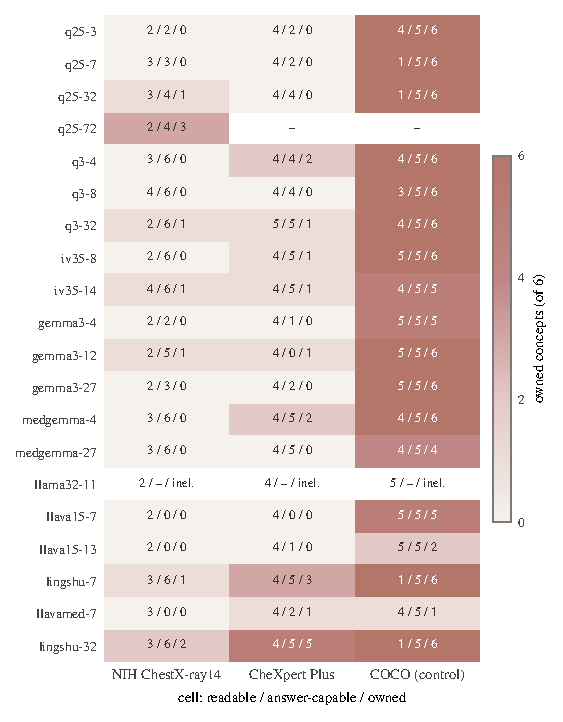
\includegraphics[width=0.7\textwidth]{figures/cf_F1_leaderboard_heatmap.pdf}
    \caption{Leaderboard heat map: owned concepts per checkpoint and dataset, annotated with readable/answerable/owned counts.}
    \label{fig:cf-heatmap}
\end{figure}

\begin{figure}[h]
    \centering
    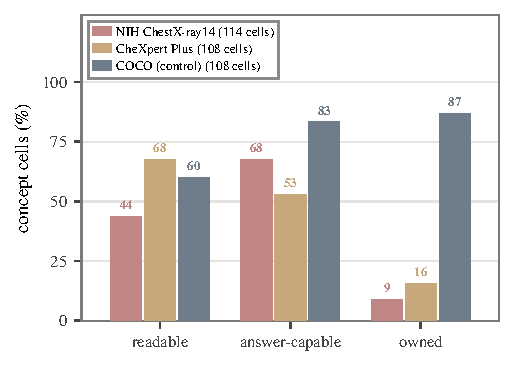
\includegraphics[width=0.55\textwidth]{figures/cf_F8_capability_counts.pdf}
    \caption{Fraction of concept cells that are readable, answerable, and owned, per dataset.}
    \label{fig:cf-counts}
\end{figure}

\begin{figure}[h]
    \centering
    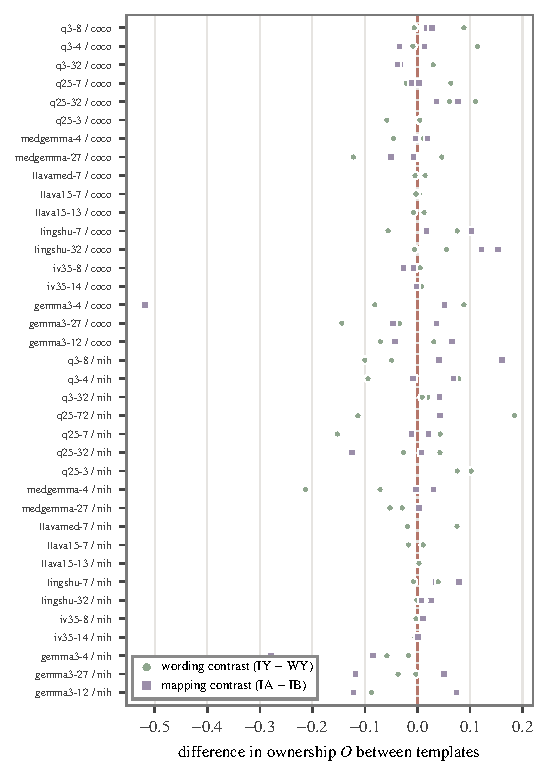
\includegraphics[width=0.7\textwidth]{figures/cf_F10_prompt_dependence.pdf}
    \caption{Wording (IY$-$WY) and mapping (IA$-$IB) contrasts of ownership for every block with the PROMPT module.}
    \label{fig:cf-prompt}
\end{figure}
